\documentclass[a4paper,11pt]{article}
\usepackage{a4wide}
\usepackage{fullpage}
\usepackage[utf8x]{inputenc}
%\usepackage[slovene]{babel}
%\selectlanguage{slovene}
\usepackage[toc,page]{appendix}
\usepackage[pdftex]{graphicx} 
\usepackage{amsfonts}
\usepackage{amsmath}
\usepackage{setspace}
\usepackage{color}
\definecolor{light-gray}{gray}{0.95}
\usepackage{listings} 
\usepackage{hyperref}
\renewcommand{\baselinestretch}{1.2} 
\renewcommand{\appendixpagename}{Priloge}

\lstset{ 
language=Python,
basicstyle=\footnotesize,
basicstyle=\ttfamily\footnotesize\setstretch{1},
backgroundcolor=\color{light-gray},
}

\title{Topological data analysis \\ Homework 1}
\author{Sara Bizjak (27202020)}
\date{\today}

\begin{document}

\maketitle

\section{Theoretical problems}
\subsection{Exploring different metrics}

%%%%%%%%%%%%%%%%%%%%%%%%%%%%%%%%%%%%%%%%%%%%%%%%%%%%%%%%%%%%%%%%%%%%%%%%%%%%%%%%

a) Determing the distances between the points $(2, 1), \ (4, 2), \ (0, 2)$ in metrics $\alpha, \  \beta, \ \gamma$.

\begin{itemize}
    \item Metric $\alpha$.
        
    \begin{equation*}
        \text{d}_{\alpha} \big( (2, 1), \ (4, 2) \big) = \sqrt{2^2 + 1^2} + \sqrt{4^2 + 2^2} = \sqrt{5} + \sqrt{20} = 6.708203932499369.
    \end{equation*}

    \begin{equation*}
        \text{d}_{\alpha} \big( (2, 1), \ (0, 2) \big) = \sqrt{2^2 + 1^2} + \sqrt{0^2 + 2^2} = \sqrt{5} + \sqrt{4} = 4.23606797749979.
    \end{equation*}

    \begin{equation*}
        \text{d}_{\alpha} \big( (4, 2), \ (0, 2) \big) = \sqrt{4^2 + 2^2} + \sqrt{0^2 + 2^2} = \sqrt{20} + \sqrt{4} = 6.47213595499958.
    \end{equation*}

%%%%%%%%%%%%%%%%%%%%%%%%%%%%%%%%%%%%%%%%%

    \item Metric $\beta$.
    
    \begin{equation*}
        \text{d}_{\beta} \big( (2, 1), \ (4, 2) \big) = \sqrt{(2 - 4)^2 + (1 - 2)^2} = \sqrt{4 + 1} = 2.23606797749979.
    \end{equation*}
        
    \begin{equation*}
        \text{d}_{\beta} \big( (2, 1), \ (0, 2) \big) = \sqrt{2^2 + 1^2} + \sqrt{0^2 + 2^2} = \sqrt{5} + \sqrt{4} = 4.23606797749979.
    \end{equation*}
        
    \begin{equation*}
        \text{d}_{\beta} \big( (4, 2), \ (0, 2) \big) = \sqrt{4^2 + 2^2} + \sqrt{0^2 + 2^2} = \sqrt{20} + \sqrt{4} = 6.47213595499958.
    \end{equation*}

%%%%%%%%%%%%%%%%%%%%%%%%%%%%%%%%%%%%%%%%%

    \item Metric $\gamma$.
    
    \begin{equation*}
        \text{d}_{\gamma} \big( (2, 1), \ (4, 2) \big) = |2 - 4| + |1| + |2| = 2 + 1 + 2 = 5.
    \end{equation*}
        
    \begin{equation*}
        \text{d}_{\gamma} \big( (2, 1), \ (0, 2) \big) = |2 - 0| + |1| + |2| = 5.
    \end{equation*}
        
    \begin{equation*}
        \text{d}_{\gamma} \big( (4, 2), \ (0, 2) \big) = |4 - 0| + |2| + |2| = 4 + 2 + 2 = 8.
    \end{equation*}


\end{itemize}

%%%%%%%%%%%%%%%%%%%%%%%%%%%%%%%%%%%%%%%%%%%%%%%%%%%%%%%%%%%%%%%%%%%%%%%%%%%%%%%%

b) Drawing the open balls $B \big((0, 0), 1 \big)$, $B \big((1, 0), 2 \big)$, $B \big((0, 2), 6 \big)$ in $\alpha$ metric. 

\begin{align*} 
    B \big((0, 0), 1 \big) &= \{(0,0)\} \cup \{(x,y) \in \mathbb{R}^2 : \sqrt{x^2 + y^2} + \sqrt{0^2 + 0^2}< 1 \} 
    \\
    &= \{(0,0)\} \cup \{(x,y) \in \mathbb{R}^2 : \sqrt{x^2 + y^2} < 1 \}. 
\end{align*}

\begin{figure}[ht!]
    \centering
    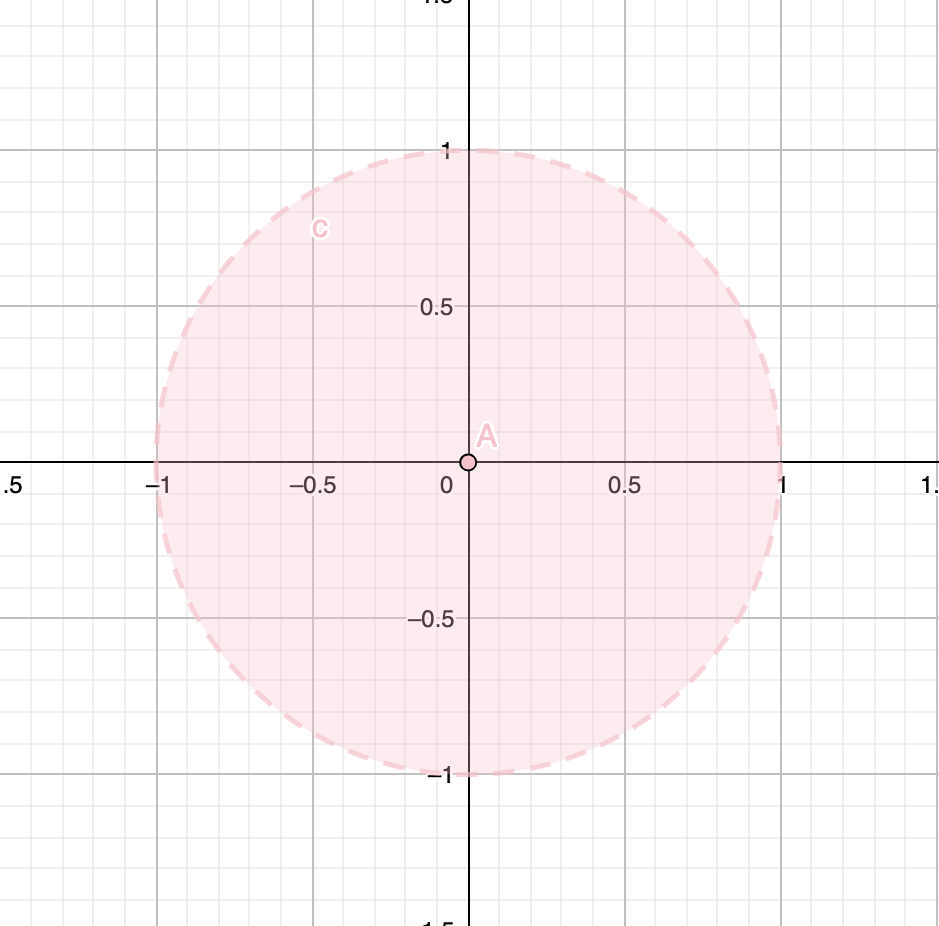
\includegraphics[width=60mm]{b1.png}
    \caption{$B \big((0, 0), 1 \big)$ in metric $\alpha$.}
\end{figure}

%%%%%%%%%%%%%%%%%%%%%%%%%%%%%%%%%%%%%%%%%%

\begin{align*} 
    B \big((1, 0), 2 \big) &= \{(1,0)\} \cup \{(x,y) \in \mathbb{R}^2 \setminus (1,0) : \sqrt{x^2 + y^2} + \sqrt{1^2 + 0^2} < 2 \}
    \\
    &= \{(1,0)\} \cup \{(x,y) \in \mathbb{R}^2 \setminus (1,0) : \sqrt{x^2 + y^2} < 1 \} .
\end{align*}

\begin{figure}[ht!]
    \centering
    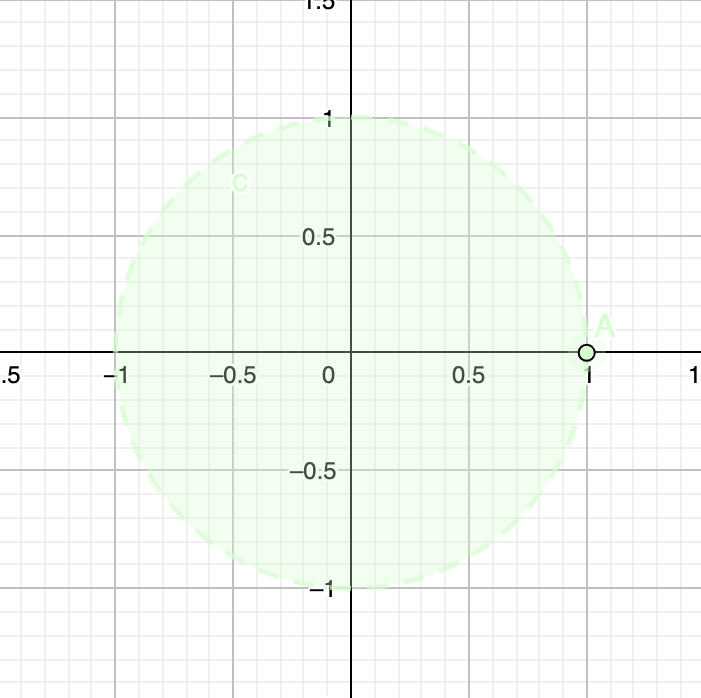
\includegraphics[width=60mm]{b2.png}
    \caption{$B \big((1, 0), 2 \big)$ in metric $\alpha$.}
\end{figure}

 %%%%%%%%%%%%%%%%%%%%%%%%%%%%%%%%%%%%%%%%%

 \begin{align*} 
    B \big((0, 2), 6 \big) &= \{(0,2)\} \cup \{(x,y) \in \mathbb{R}^2 \setminus (0,2) : \sqrt{x^2 + y^2} + \sqrt{0^2 + 2^2} < 6 \} 
    \\
    &= \{(0,2)\} \cup \{(x,y) \in \mathbb{R}^2 \setminus (0,2) : \sqrt{x^2 + y^2} < 4 \}. 
\end{align*}

\begin{figure}[ht!]
    \centering
    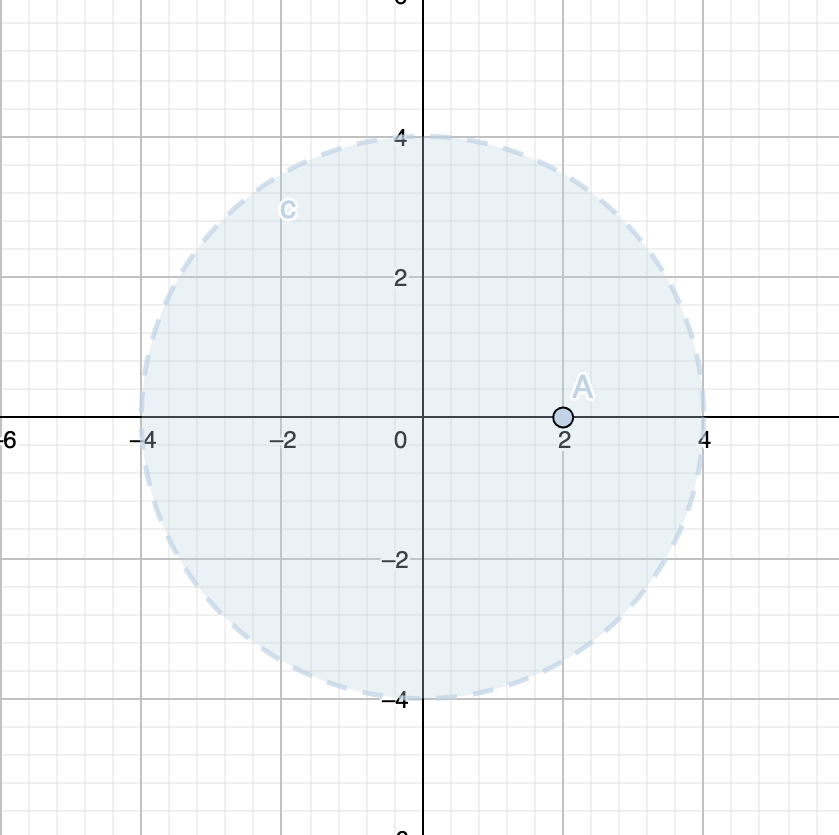
\includegraphics[width=60mm]{b3.png}
    \caption{$B \big((0, 2), 6 \big)$ in metric $\alpha$.}
\end{figure}
%%%%%%%%%%%%%%%%%%%%%%%%%%%%%%%%%%%%%%%%%%%%%%%%%%%%%%%%%%%%%%%%%%%%%%%%%%%%%%%%%%%%%%

c) Drawing the open balls $B \big((0, 0), 1 \big)$, $B \big((1, 0), 2 \big)$, $B \big((2, 2), 3 \sqrt{2} \big)$ in $\beta$ metric. 

\begin{align*} 
    B \big((0, 0), 1 \big) &= \{(x,y) \in \mathbb{R}^2 : \sqrt{(x - 0)^2 + (y - 0)^2} < 1 \}
    \\
    &= \{(x,y) \in \mathbb{R}^2 : \sqrt{x^2 + y^2} < 1 \}.
\end{align*}

\begin{figure}[ht!]
    \centering
    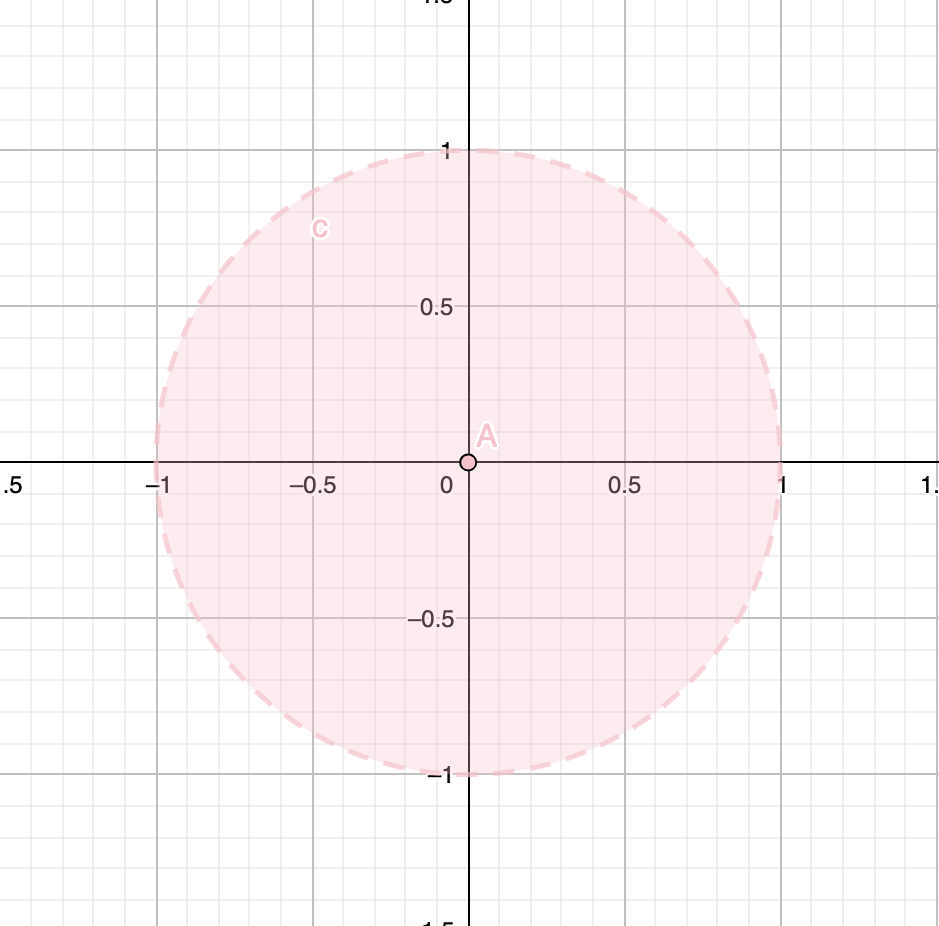
\includegraphics[width=60mm]{b1.png}
    \caption{$B \big((0, 0), 1 \big)$ in metric $\beta$.}
\end{figure}

%%%%%%%%%%%%%%%%%%%%%%%%%%%%%%%%%%%%%%%%%%%%

\begin{align*} 
    B \big((1, 0), 2 \big) &= \{(x,0) \in \mathbb{R}^2 : \sqrt{(x - 1)^2} < 2 \} \cup \{(x, y) \in \mathbb{R}^2, \ y \neq 0 : \sqrt{x^2 + y^2} + \sqrt{1^2} < 2 \}
    \\
    &= \{(x,0) \in \mathbb{R}^2 : |x - 1| < 2 \} \cup \{(x,y) \in \mathbb{R}^2, \ y \neq 0 : \sqrt{x^2 + y^2} < 1 \} 
    \\
    &= \{(x,0) \in \mathbb{R}^2 : -1 < x < 3 \} \cup \{(x,y) \in \mathbb{R}^2, \ y \neq 0 : \sqrt{x^2 + y^2} < 1 \} .
\end{align*}

\begin{figure}[ht!]
    \centering
    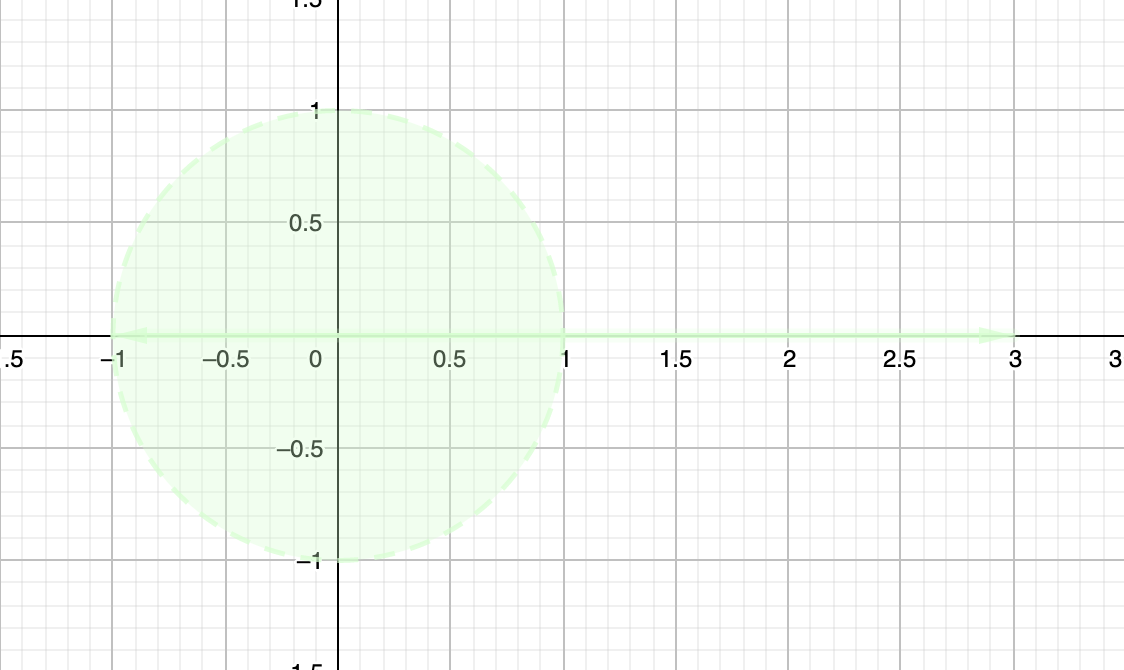
\includegraphics[width=40mm]{c2.png}
    \caption{$B \big((1, 0), 2 \big)$ in metric $\beta$.}
\end{figure}

 %%%%%%%%%%%%%%%%%%%%%%%%%%%%%%%%%%%%%%%%%%%

\begin{align*} 
    B \big((2, 2), 3 \sqrt{2} \big) &= \{(x,x) \in \mathbb{R}^2 : \sqrt{2 \cdot (x - 2)^2} < 3 \sqrt{2} \} \cup \{(x, y) \in \mathbb{R}^2, \ x \neq y : \sqrt{x^2 + y^2} + \sqrt{2 \cdot 2^2} < 3 \sqrt{2} \}
    \\
    &= \{(x,x) \in \mathbb{R}^2 : \sqrt{2} \cdot |x - 2| < 3 \sqrt{2} \} \cup \{(x,y) \in \mathbb{R}^2, \ x \neq y : \sqrt{x^2 + y^2} + 2 \sqrt{2} < 3 \sqrt{2} \} 
    \\
    &= \{(x,x) \in \mathbb{R}^2 : -1 < x < 5\} \cup \{(x,y) \in \mathbb{R}^2, \ x \neq y : \sqrt{x^2 + y^2} < \sqrt{2} \} .
\end{align*}

\begin{figure}[ht!]
    \centering
    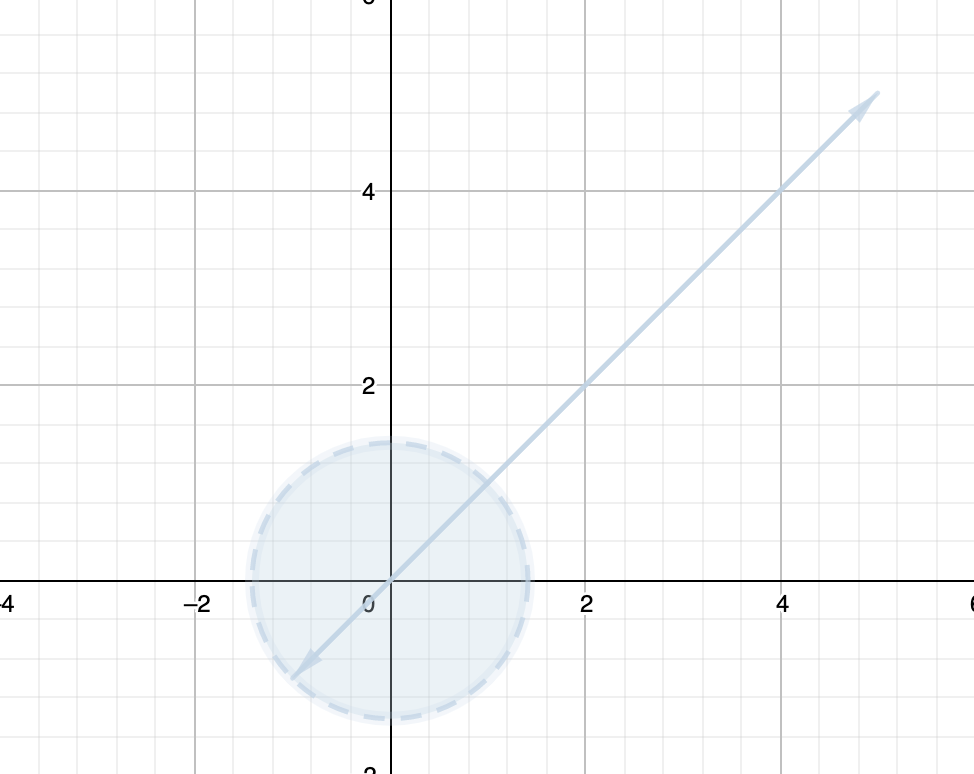
\includegraphics[width=60mm]{c3.png}
    \caption{$B \big((2, 2), 3 \big)$ in metric $\beta$.}
\end{figure}

%%%%%%%%%%%%%%%%%%%%%%%%%%%%%%%%%%%%%%%%%%%%%%%%%%%%%%%%%%%%%%%%%%%%%%%%%%%%%%%%%%%%%%%%%%%%%

d) Drawing the open balls $B \big((0, 0), 1 \big)$, $B \big((1, 0), 2 \big)$, $B \big((2, 0), 3  \big)$ in $\gamma$ metric. 

\begin{align*} 
    B \big((0, 0), 1 \big) &= \{(0,y) \in \mathbb{R}^2 : |y - 0| < 1 \} \cup \{(x,y) \in \mathbb{R}^2 , \ x \neq 0: |x - 0| + |y - 0| < 1 \}
    \\
    &= \{(0,y) \in \mathbb{R}^2 : -1 < y < 1 \} \cup \{(x,y) \in \mathbb{R}^2 : -1 < x < 1, \ -1 < y < 1 \}.
\end{align*}

\begin{figure}[ht!]
    \centering
    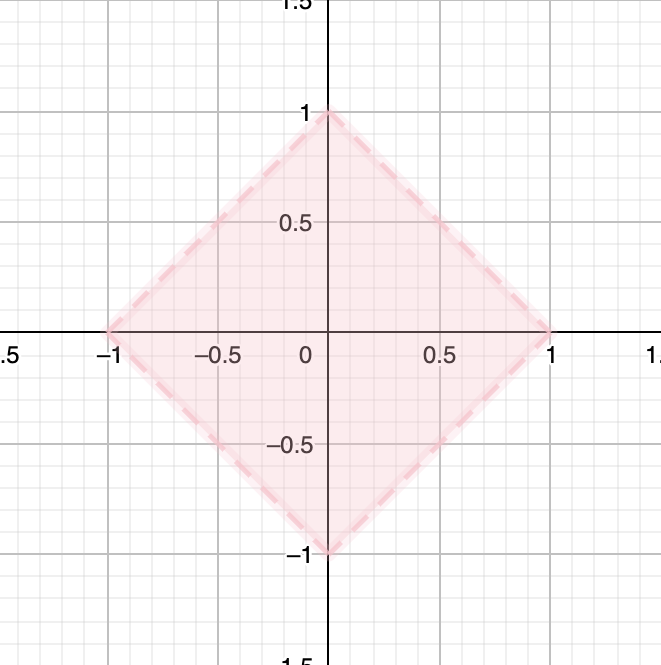
\includegraphics[width=60mm]{d1.png}
    \caption{$B \big((0, 0), 1 \big)$ in metric $\gamma$.}
\end{figure}

%%%%%%%%%%%%%%%%%%%%%%%%%%%%%%%%%%%%%%%%%%%%
\begin{align*} 
    B \big((1, 0), 2 \big) &= \{(1,y) \in \mathbb{R}^2 : |y - 0| < 2 \} \cup \{(x,y) \in \mathbb{R}^2, \ x \neq 1 : |x - 1| + |y - 0| < 2 \}
    \\
    &= \{(1,y) \in \mathbb{R}^2 : -2 < y < 2 \} \cup \{(x,y) \in \mathbb{R}^2 , \ x \neq 1: -1 < x < 3, \ -2 < y < 2 \}.
\end{align*}

\begin{figure}[ht!]
    \centering
    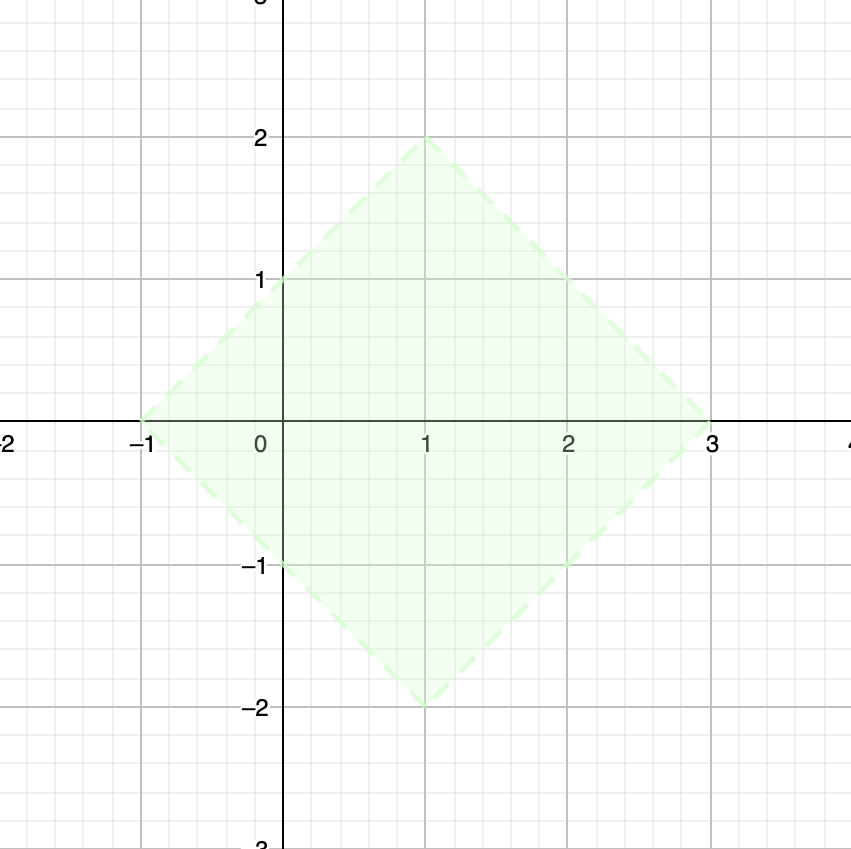
\includegraphics[width=60mm]{d2.png}
    \caption{$B \big((1, 0), 2 \big)$ in metric $\gamma$.}
\end{figure}

 %%%%%%%%%%%%%%%%%%%%%%%%%%%%%%%%%%%%%%%%%%%
\begin{align*} 
    B \big((2, 0), 3 \big) &= \{(2,y) \in \mathbb{R}^2 : |y - 0| < 3 \} \cup \{(x,y) \in \mathbb{R}^2, \ x \neq 2 : |x - 2| + |y - 0| < 3 \}
    \\
    &= \{(2,y) \in \mathbb{R}^2 : -3 < y < 3 \} \cup \{(x,y) \in \mathbb{R}^2 , \ x \neq 2: -1 < x < 5, \ -3< y < 3 \}.
\end{align*}

\begin{figure}[ht!]
    \centering
    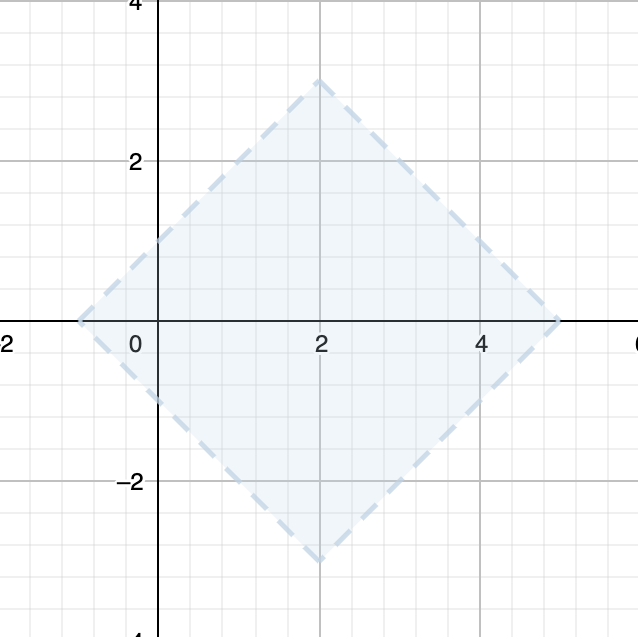
\includegraphics[width=60mm]{d3.png}
    \caption{$B \big((2, 0), 3 \big)$ in metric $\gamma$.}
\end{figure}



%%%%%%%%%%%%%%%%%%%%%%%%%%%%%%%%%%%%%%%%%%%%
\end{document}



